\begin{figure}[htbp]
\centering
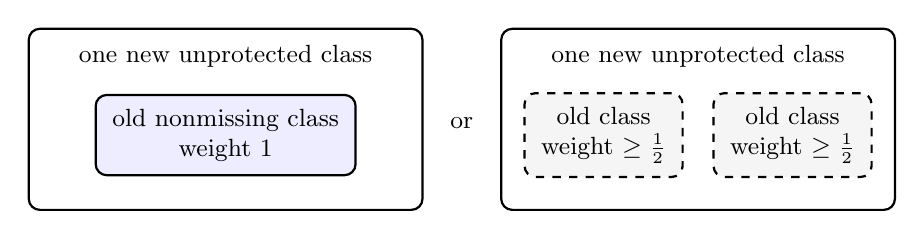
\begin{tikzpicture}[font=\small,thick]
 \draw[rounded corners] (0,0) rectangle (5,2.3);
 \draw[rounded corners] (6,0) rectangle (11,2.3);
 \node at (2.5,1.95) {one new unprotected class};
 \node at (8.5,1.95) {one new unprotected class};
 \node[draw,rounded corners,fill=blue!7,align=center,
       inner xsep=6pt,inner ysep=5pt] at (2.5,0.95)
       {old nonmissing class\\weight $1$};
 \node[draw,dashed,rounded corners,fill=black!4,align=center,
       inner xsep=6pt,inner ysep=5pt] at (7.3,0.95)
       {old class\\weight $\ge\frac12$};
 \node[draw,dashed,rounded corners,fill=black!4,align=center,
       inner xsep=6pt,inner ysep=5pt] at (9.7,0.95)
       {old class\\weight $\ge\frac12$};
 \node at (5.5,1.1) {or};
\end{tikzpicture}
\caption{The weighted containment argument in the chain bound. All
classes shown have one fixed sign and contain no protected label.
Each new class contains either a whole nonmissing old class or two
distinct whole old classes. A missing old class has weight $1/2$;
every other old class has weight $1$. The displayed regions express
set containment schematically. Distinct new classes cannot use the
same whole old class, so their unit weight requirements add.}
\label{fig:nesting-budget}
\end{figure}
